\documentclass[11pt,dvipdfmx]{jsarticle}
\usepackage{amsmath,amsfonts}
\usepackage{titlesec}
\usepackage{graphicx}
\usepackage{float}
\usepackage{comment}
\usepackage{fancyhdr}
\usepackage{url}
\usepackage[dvipdfmx]{hyperref}
\usepackage{pxjahyper}

\usepackage{setspace}

\usepackage{siunitx}

\usepackage[final]{pdfpages}

%\lhead{}%ヘッダ左上を空白化
\graphicspath{{../fig/}}%\includegraphicsのファイル名省略用

%高さの設定
\setlength{\textheight}{\paperheight}%ひとまず紙面を本文領域に
\setlength{\topmargin}{-5.4truemm}%上の余白を20mm(=1inch-5.4mm)に
\addtolength{\topmargin}{-\headheight}%
\addtolength{\topmargin}{-\headsep}%ヘッダの分だけ本文領域を移動させる
\addtolength{\textheight}{-40truemm}%下の余白も20mmに
%%幅の設定
\setlength{\textwidth}{\paperwidth}%ひとまず紙面を本文領域に
\setlength{\oddsidemargin}{-0.4truemm}%左の余白を20mm(=1inch-5.4mm)に
\setlength{\evensidemargin}{-0.4truemm}%
\addtolength{\textwidth}{-50truemm}%右の余白も20mmに

%図，表の表示名
\renewcommand{\figurename}{Fig. }
\renewcommand{\tablename}{Table }

%図，表，式などの間隔
\setlength{\abovecaptionskip}{1mm}	%図・表とキャプションの間隔の変更
\setlength{\belowcaptionskip}{1mm}
\setlength{\abovedisplayskip}{3pt}%式の上部のマージン
\setlength{\belowdisplayskip}{3pt}%式の下部のマージン

%図番号を(subsection).(図番号)に変更
\makeatletter
\renewcommand{\thefigure}{\thesection.\arabic{figure}}
\@addtoreset{figure}{section}

%表番号を(subsection).(表番号)に変更
\renewcommand{\thetable}{\thesection.\arabic{table}}
\@addtoreset{table}{section}

%式番号を(subsection).(式番号)に変更
\renewcommand{\theequation}{\thesection.\arabic{equation}}
\@addtoreset{equation}{section}
\makeatother

%注釈
\renewcommand\thefootnote{*\arabic{footnote}}

%目次の表示レベル設定
\setcounter{tocdepth}{3}

\renewcommand{\postpartname}{章} %部を章に変更

\begin{document}

\begin{titlepage}
  \begin{center}

    \vspace{20mm}
    {\Large 千葉工業大学}\\
    \vspace{5mm}
    {\Large 学位論文}\\
		\vspace{65mm}
    {\huge 方向可変な車輪を有する\\\vspace{5mm}8輪運搬ロボットの開発}\\
    \vspace{3mm}
    {\Large Development of an 8-wheeled transport robot with variable-direction wheels}\\
    \vspace{65mm}
		{\Large 2026年1月}\\
    \vspace{10mm}
    {\Large 所属：未来ロボティクス学科}\\
    \vspace{5mm}
    {\Large 学生番号: 22C1089}\\
    {\Large 氏名：床枝純}\\
    \vspace{5mm}
    {\Large 指導教員：米田 完 教授}
    
  \end{center}

\end{titlepage}

\pagestyle{empty}

%アブストラクト
\vspace*{20mm} % ページ上部の余白調整
\renewcommand{\abstractname}{\LARGE 要旨}
\begin{abstract}
  \vspace{5mm}
  本研究は，日本橋梁株式会社との共同研究として，
  鋼橋の塗膜剥離作業を自動化するための磁気吸着式壁面走行システムの開発を目的としたものである．

  現在，鋼橋の塗り替えにおける塗膜剥離作業は，
  高所かつ過酷な環境下での手作業に依存しており，
  作業者の負担軽減が急務となっている．
  先行研究では，
  高周波誘導加熱（IH）を用いて塗膜を浮かせ，
  剥離を容易にする装置や走行ロボットが開発されてきたが，
  最終的なスクレーパによる剥離工程は依然として手作業による部分が多い．

  本研究では，
  剥離作業時の安定性を確保するため，
  2輪駆動と1つのフリーローラによる三点支持構造を採用した専用の移動機体を開発した．
  本システムは20個のネオジム磁石を備え，
  壁面との間に5mmの距離を保持して走行する設計となっている．

  実橋梁でのフィールドテストの結果，
  自走による剥離試行時にスクレーパが受ける反力によって機体前方が壁面から浮上し，
  スタック（走行不能）となる現象が確認された．
  一方で，手動による初期切削を行った後では，
  自走による安定した剥離が可能であることを確認した．

  本研究の成果および共同研究先からの知見により，
  自動剥離の完全実現には，
  刃先の貫入角度40度から剥離角度10度へ動的に刃角を制御する機構の実装が極めて重要であることが示唆された．
\end{abstract}

\newpage
%目次
\pagestyle{fancy}
\renewcommand{\footrulewidth}{0.4pt}%フッターラインの線幅の変更。デフォルトは0.4pt
\pagenumbering{Roman}		%ページ番号をローマ数字に
\tableofcontents

\vspace{5mm}
%\leftline{\textgt{付録A: フレーム部品外注図面}}


\newpage
%図目次の表示
\listoffigures
%表目次の表示dd
\listoftables

\clearpage
\setcounter{page}{1}
\pagenumbering{arabic}	%ページ番号をアラビア数字に

%第1章
%第1章
\part{序論}
\label{zyoron}

\section {ニューマチックケーソン工法における作業の無人化}
\subsection{研究背景}

近年, 危険な場所での作業による事故などを無くすため, 急速に作業の機械化・無人化が進められてきた.
ロボットは人の代わりとなり, 様々な作業を効率良く行うツールとしてこれまで広く普及されてきたが, 現場環境に応じた様々な問題点も挙げられている.

\subsubsection{ニューマチックケーソン工法とは}

橋梁や建物の基礎の構築に使用される工法として, ニューマチックケーソン工法が挙げられる.

ニューマチックケーソン工法とは, 地上に構築した構造物の直下を掘削・排土する事で, 地下に沈設する工法である.
地上に構築する構造物は函（躯体）と呼ばれ, その最下部の作業室と称する密閉された部屋に高圧な空気を送り込む事で, 地下水の侵入を防ぎ地上と同じような状態で掘削を行う事ができる利点がある.

橋梁や建物の基礎の他に, シールドトンネルの立杭や下水ポンプ場, 地下調整池, あるいは地下鉄や道路トンネルなど, 幅広く活用されている.\cite{koukyou}

\subsubsection{大深度ニューマチックケーソン工法と工法の問題点}

大深度開発事業を行うために, 水面下70[m]までの地下構造物の構築を可能にする工法を大深度ニューマチックケーソン工法（以下ケーソン工法）と呼ぶ.
沈設方法はニューマチックケーソン工法と同様であるが, 理論作業気圧を0.7[MPa]まで上げる事で, より深くに地下構造物の構築する事を可能にしている.
しかし作業気圧が0.4[MPa]を超える工事は, 減圧症や高気圧障害の発生リスクがある為, 作業の無人化が求められている.
ケーソン工法の概要を図\ref{ke-son1}に示す.\cite{paint}

\begin{figure}[H]
	\centering
	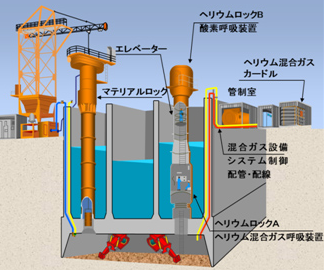
\includegraphics[width=0.60\textwidth]{ke-son_gaiyo.png}
	\caption{Overview of deep pneumatic caisson construction method\cite{paint}}
	\label{ke-son1}
\end{figure}

\newpage


\subsection{先行機体}
\subsubsection{クローラ型移動ロボット}
現在作業空間内ではクローラ型移動ロボットが作業を行っている.
図\ref{sennkou1}, \ref{sennkou2}に示す.


\begin{figure}[H]
  \begin{minipage}{0.5\hsize}
    \centering
    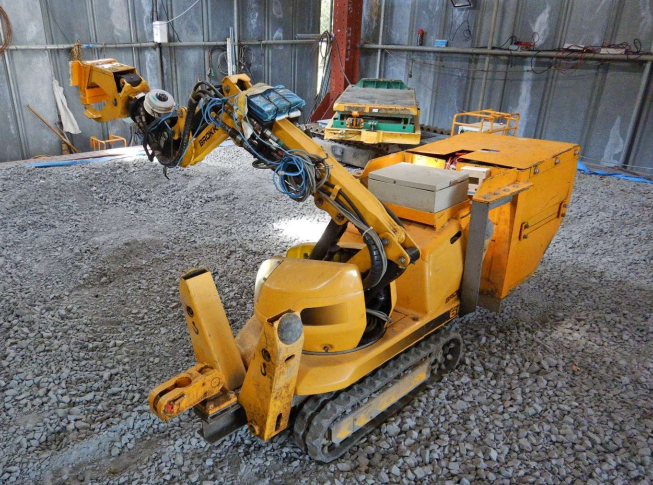
\includegraphics[height=50mm]{sennkoukitai1.png}
    \caption{Demolition robot\cite{youtuu}}
    \label{sennkou1}
  \end{minipage}
  \begin{minipage}{0.5\hsize}
    \centering
    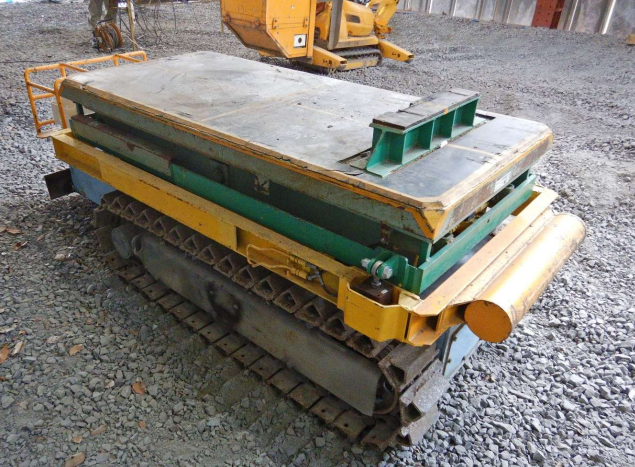
\includegraphics[height=50mm]{sennkoukitai2.png}
    \caption{Transportation robot\cite{youtuu}}
    \label{sennkou2}
  \end{minipage}
\end{figure}


\subsubsection{スタックを起こす原因}
クローラ型移動ロボットは, 駆動部の進行方向に対して高い踏破性能を持ち, 不整地での走行において広く普及している.

しかしクローラ型移動ロボットは, 機体側面の障害物に対しての踏破性能が低いという問題点がある.
また, クローラ型移動ロボットは超信地旋回という旋回方式を取るが, 泥濘地で超信地旋回を行うと地面を掘ってしまい, 弱点である機体側面に障害物を生成してしまう.

よって現行のロボットは機体側面に生じた障害によりスタックを起こすと推測できる.

クローラ型移動ロボットがスタックを起こしている状態を図\ref{sennkou3}に示す.

\begin{figure}[H]
	\centering
	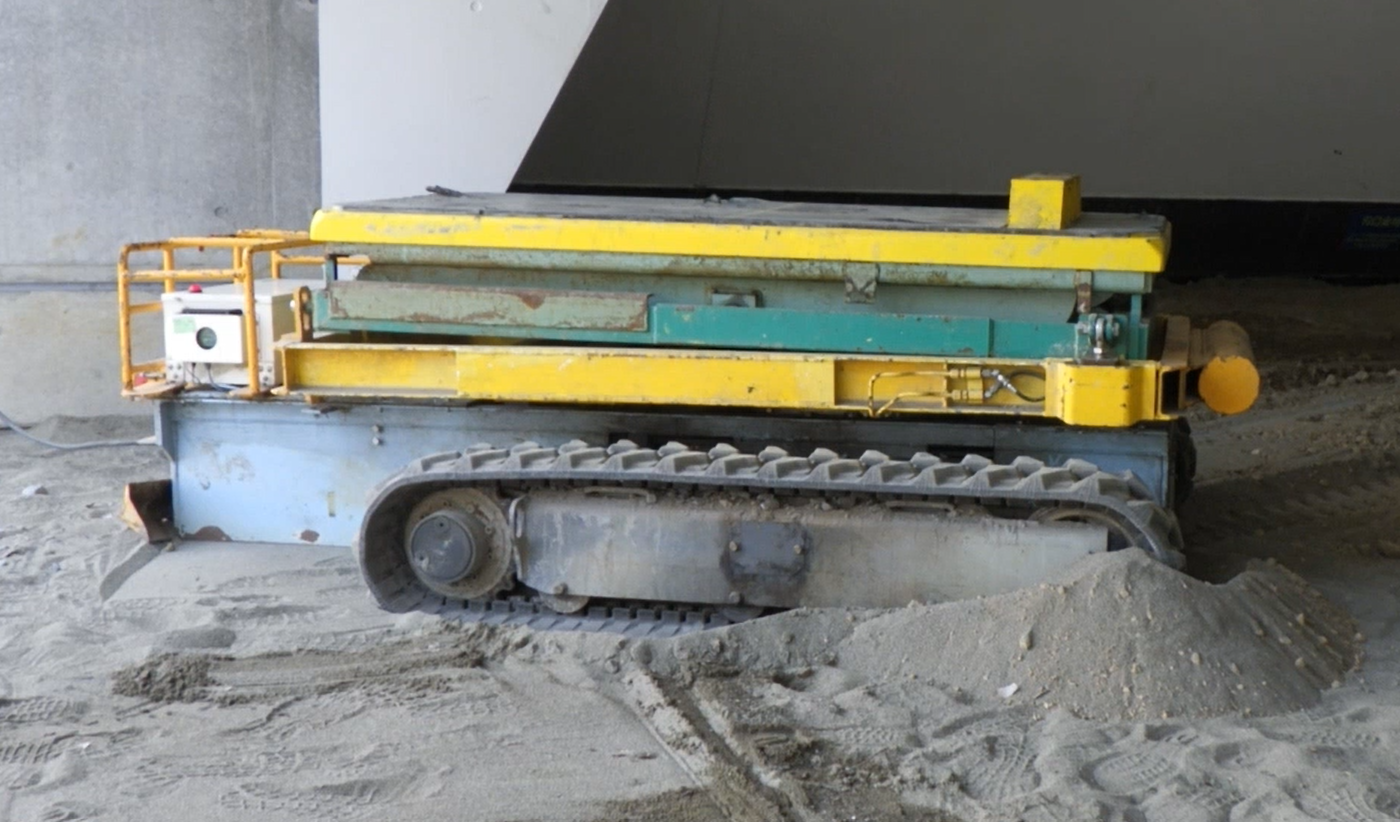
\includegraphics[width=0.7\textwidth]{stack1.png}
  \caption{robot stuck\cite{ih-catalog}}
	\label{sennkou3}
\end{figure}

\newpage

\subsection{研究目的}
作業空間は圧力により地下水の侵入を防いでいるため泥濘地である場合があり, また掘削による起伏や溝などの存在も想定される.

現在も作業空間内ではロボットが作業を行っているが, 上記の理由からスタックを起こす事があり復旧には人手を要するため, 作業の無人化が滞っている.

作業空間内でスタックを起こす事が無くなれば作業の無人化に大きく近づく為, 本研究では作業空間内で想定される環境でスタックを起こさないロボットの開発を研究目的とする.
作業空間内の状態の一例を図\ref{ke-son2}に示す.\cite{ih-group}


\begin{figure}[H]
	\centering
	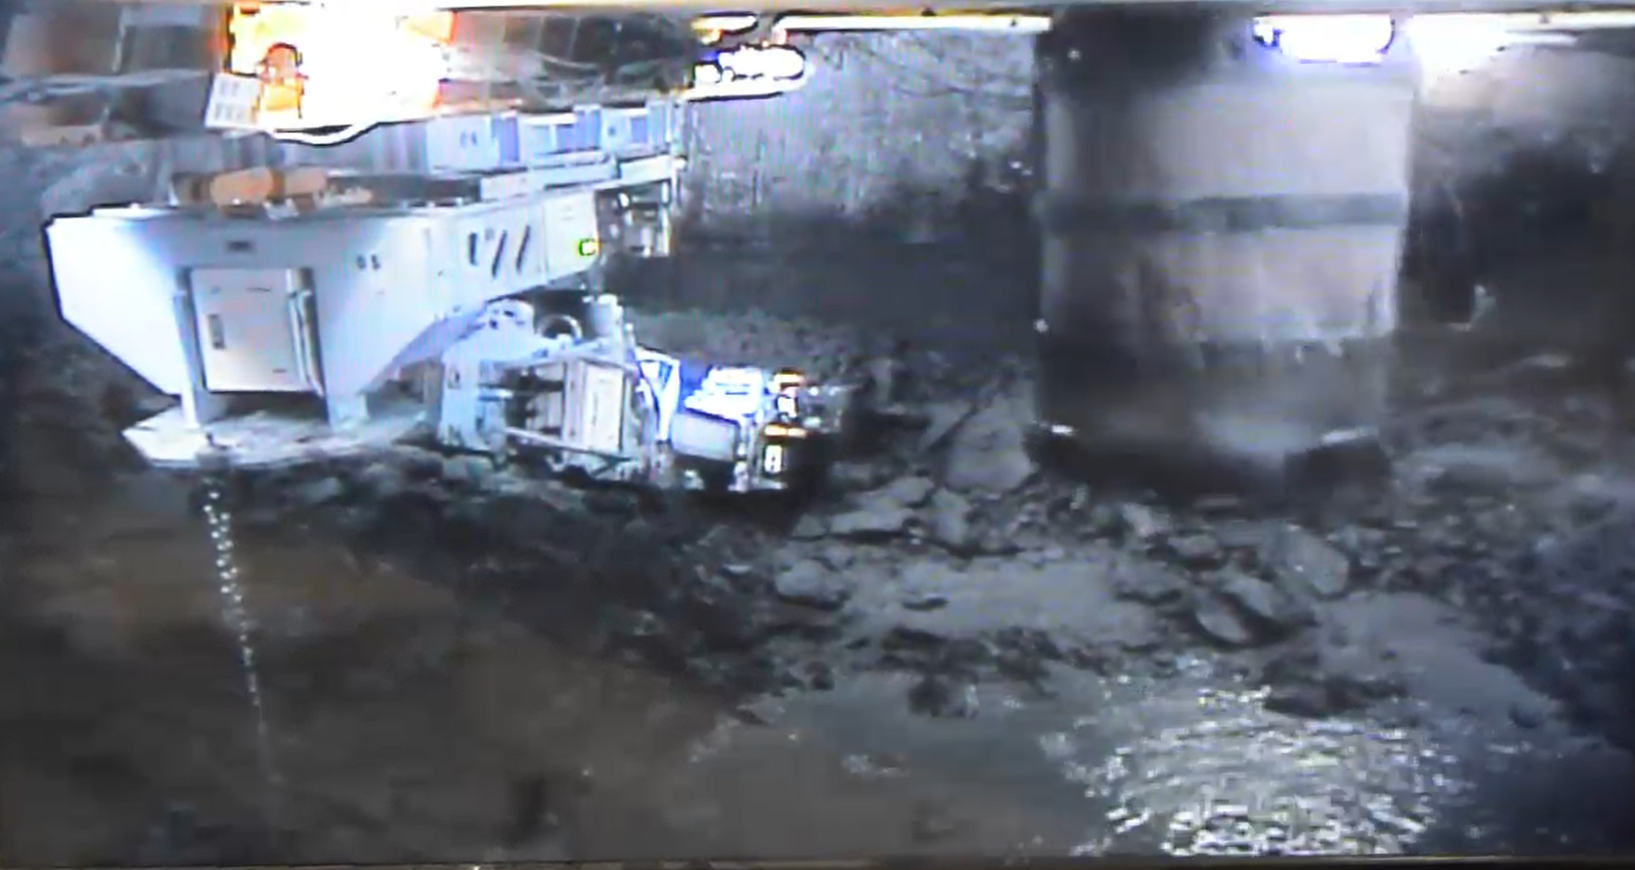
\includegraphics[width=1.0\textwidth]{ke-son_kankyo.png}
  \caption{Condition inside the work room\cite{ih-group}}
	\label{ke-son2}
\end{figure}

\subsection{本書の構成}
本論文は5章構成となっている.
第1章ではニューマチックケーソン工法の概要と先行機体の問題点を指摘し, 本研究の目的を提示した.

第2章では目的を達成する為に過去に取り組まれた研究とその問題点に対して言及し, 本研究の目標を説明する.

第3章では目標の達成を目指した機体の構想を提示し, 設計図を示したのちに製作機体の説明をする.

第4章では製作した機体を使用し, 研究目標が達成可能かの実験についての説明をし, 実験結果と考察を論じる.

第5章では本論の結論と今後の展望について説明する.





%第2章
% 第2章
\part{壁面走行システムの設計と製作}
\label{design}

\section{機体コンセプトと足回り機構}

\subsection{機体諸元}
機体の主要諸元は以下の通りである．
  \begin{table}[h]
      \centering
      \caption{Specifications of the system} % ここで自動的に Table 1 と表示されます
      \label{tab:spec}
      \begin{tabular}{ll}
      \hline
      Size           & 400 $\times$ 300 $\times$ 200 (\,mm) \\ \hline
      Weight         & 8.18 (\,kg) \\ \hline
      Motor          & DC Motor (MS-555VC) $\times$ 2 \\ \hline
      Power source   & \begin{tabular}[c]{@{}l@{}}Li-Poly Battery\\ (14.8V, 4000mAh, 100C)\end{tabular} \\ \hline
      Wheels         & \begin{tabular}[c]{@{}l@{}}Urethane Wheels\\ (ROEKGA100-20-50-T10) $\times$ 2\end{tabular} \\ \hline
      Controller     & \begin{tabular}[c]{@{}l@{}}Wireless Controller\\ (PS4 DualShock 4)\end{tabular} \\ \hline
      \end{tabular}
 \end{table}
  

\newpage

\subsection{三点支持構造による接地安定性の確保}
壁面走行ロボットにおいて，
全車輪が常に壁面に接地しトルクを伝達することは，
安全な走行を実現する上で不可欠である．
一般的な四輪構造では，壁面に微細な不陸（凹凸）が存在する場合，
対角の車輪が浮き上がる「がたつき」が生じやすい．
本研究では，これを解決するために2つの駆動輪と1つのフリーローラからなる三点支持構造を採用した．
三点支持は幾何学的に常に一つの平面を決定する静定構造であるため，
複雑なサスペンション機構を用いることなく常に全車輪が接地し，
安定した接地圧を確保することが可能である．

\begin{figure}[H] 
  \centering 
  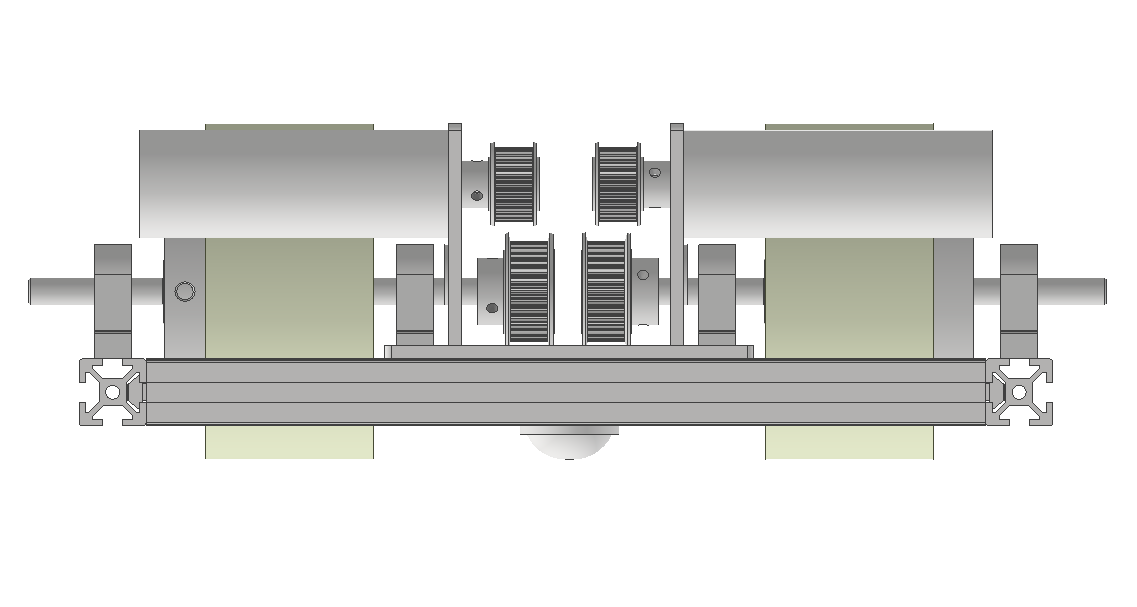
\includegraphics[width=0.6\textwidth]{santen.png} 
  \vspace{-2mm} 
  \caption{Three-point support mechanism using industrial urethane rollers} \label{fig:result} 
  \end{figure}

\newpage


\subsection{産業用ウレタンローラの採用と選定理由}
駆動輪およびフリーローラには，
産業用規格品のウレタンローラを採用した．
これは，以下の実務的な観点に基づいた選定である．
\begin{itemize}
    \item \textbf{高いグリップ力：} 鋼材壁面に対して高い摩擦係数を持つウレタンは，剥離反力に抗して機体を前進させるのに適している．
    \item \textbf{耐摩耗性とメンテナンス性：} 実橋梁の現場は錆や研削材が飛散する過酷な環境である．摩耗した際に，汎用品として安価かつ迅速に交換できるメンテナンス性の高さ（ミスミ等での入手性）を重視した．
    \item \textbf{衝撃吸収：} 適度な弾性により，段差乗り越え時の衝撃を和らげる効果がある．
\end{itemize}

\newpage

\subsection{ベルト駆動方式の採用}
動力伝達にはタイミングベルトを用いた間接駆動方式を採用した．
モータ軸と車輪軸を分離することで，機体内部のスペースを有効活用し，
重心を低く抑える設計とした．
また，直接駆動に比べてモータへの衝撃伝達を抑えられるメリットがある．

\newpage

\section{フレーム設計と実務的知見の反映}
\subsection{アルミプロファイルによる高剛性フレーム}
機体メインフレームには，軽量かつ比強度の高いアルミプロファイルを採用した．本機体の設計にあたっては，実用的な産業用ロボットの設計指針に基づき，過酷な作業環境下でも安定した性能を維持するための以下の工夫を施している．

1. 磁気吸着荷重に対する剛性の最適化 本機体は強力なネオジム磁石により常時壁面方向へ引きつけられており，フレームには常に大きな圧縮荷重と曲げモーメントが作用する．これに対し，接合部には肉厚の大型直角ブラケットを配置することで，フレームの弾性変形を抑制し，幾何学的な直角度を徹底して確保した．これにより，駆動軸の歪みを防ぎ，安定した直進走行性能を維持している．

2. 現場におけるモジュール性とメンテナンス性 実橋梁での実験では，現場の状況に応じてセンサやスクレーパの取り付け位置を微調整する必要がある．アルミプロファイルの溝を利用したボルト締結構造を採用することで，溶接構造にはない「高い拡張性（モジュール性）」を確保した．これは，部品の破損時や機構の改良時において，現場での迅速な部品交換や位置調整を可能にし，実験の継続性を高めるための実務的な設計判断である．

\begin{figure}[H] 
  \centering 
  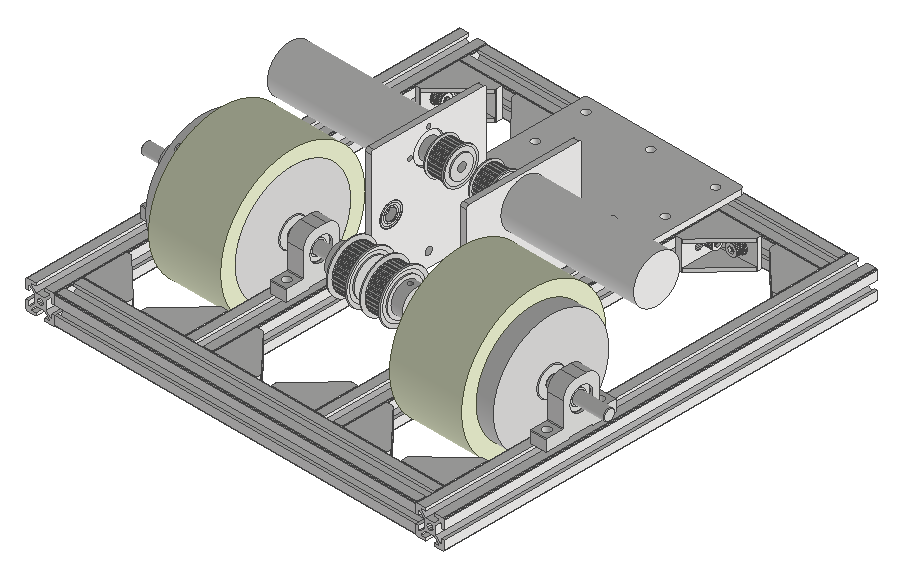
\includegraphics[width=0.6\textwidth]{ashimawari004.png} 
  \vspace{-2mm} 
  \caption{Aluminum profile frame structure and modular assembly} \label{fig:result} 
  \end{figure}
\newpage

\section{磁気吸着ユニットの設計}
\subsection{磁石配置の非対称化（12:8配置）}
本機体は合計20個のネオジム磁石（N52）を搭載している．
剥離反力は機体前方のスクレーパ部で発生し，
機体を引き剥がそうとするモーメントとして作用する．
このため，磁石配置を前方に12個，後方に8個という「非対称配置」とした．
これにより，前方の浮上を抑制する保持力を重点的に強化した．

\begin{figure}[H] 
  \centering 
  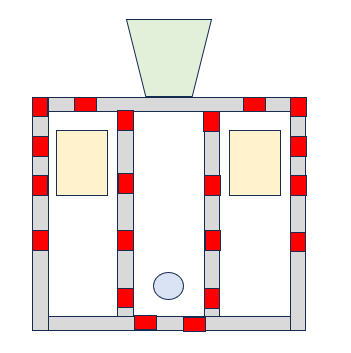
\includegraphics[width=0.6\textwidth]{haiti.png} 
  \vspace{-2mm} 
  \caption{Asymmetric layout of neodymium magnets (12 front, 8 back)} \label{fig:result} 
  \end{figure}
\newpage

\subsection{5mmの壁面距離（ギャップ）設定の根拠}
磁石面と壁面の距離は5mmに設定した．
磁石を壁面へ接近させるほど保持力は指数関数的に向上するが，
実橋梁では1mm程度の錆の隆起や塗膜の不陸が散見される．
1mm程度の距離に設定した場合，走行中に磁石ユニットがこれらに接触・激突し，
走行不能（スタック）に陥るリスクが高い．
そのため，現場環境の不確実性に対する「走破性」を優先し，
5mmという安全マージンを設定した．

\begin{figure}[H] 
  \centering 
  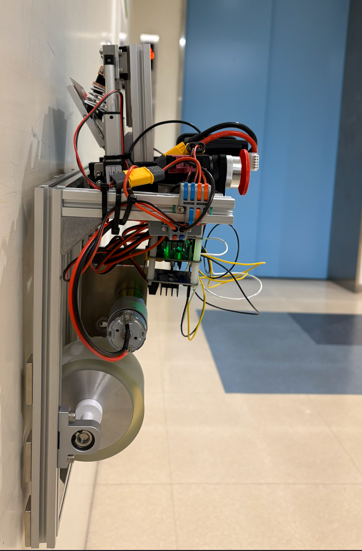
\includegraphics[width=0.6\textwidth]{gap.png} 
  \vspace{-2mm} 
  \caption{Side view of the robot showing the 5.0 mm clearance between the magnets and the wall surface} \label{fig:result} 
  \end{figure}
\newpage
%第3章
% 第3章
\part{スクレーパ機構の統合}
\label{scraper}

\section{剥離ユニットの構成}
\subsection{リニアアクチュエータによる昇降・押し込み機構}
剥離機構には，
リニアアクチュエータを用いたシリンダ駆動式スクレーパを採用した．
これは，無線コントローラからの信号により，
刃先の昇降および壁面への押し込み動作を任意に行えるものである．
作業地点までは刃を上げ，剥離開始時に強力に塗膜へ貫入させる制御を可能とした．

\begin{figure}[H] 
  \centering 
  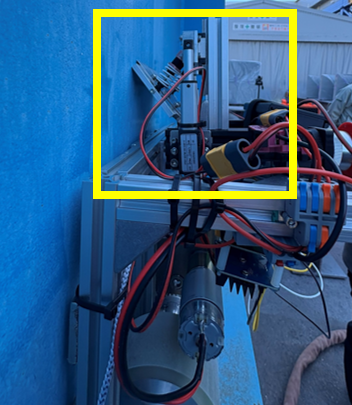
\includegraphics[width=0.6\textwidth]{tougou.png} 
  \vspace{-2mm} 
  \caption{Scraper unit integrated with DC linear actuator} \label{fig:result} 
  \end{figure}
\newpage

\section{刃先角度の設定と構造的制約}
\subsection{角度40度の採用理由}
剥離性能において，
刃先が壁面となす角度は極めて重要である．
本機体では，現行の機体フレームへの統合構造とリニアアクチュエータの可動域の兼ね合いから，
壁面接地時の刃角が約40度に固定される設計となっている．

\subsection{40度設定の力学的影響}
一般に，40度という深い角度は塗膜への「初期貫入（刺さる動作）」には非常に有利である．
しかし，貫入した状態で水平に走行しようとすると，
壁面から機体を押し返そうとする垂直方向の力（法線抗力）が大きくなる傾向がある．
この構造的制約が実際の走行にどのような影響を与えたかについて，次章で詳述する．

\newpage

%第3章
\newpage
\part{機体性能の評価実験}
今回は現場ヤードでの性能を検証するため, 想定環境での走行実験と段差踏破の実験を行った.

\section{走行実験}
研究目標でも示した通り, 現場ヤードでは以下の3つの環境が想定される.

\begin{itemize}
  \item 鉄板
  \item コンクリート
  \item アスファルト
\end{itemize}

それぞれの環境で1mの走行実験を行い, かかる時間のデータから走行性能を評価する.

実験風景を図\ref{zikkenn_image1_1}, \ref{zikkenn_image1_2}, \ref{zikkenn_image1_3}に示す.

\begin{figure}[H]
  \centering
  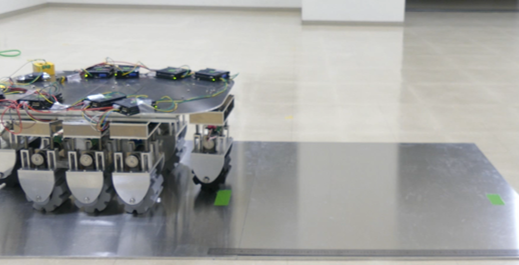
\includegraphics[width=0.8\textwidth]{zikkenn_image1.png}
  \vspace{2mm}
  \caption{Driving experiment on iron plate}
  \label{zikkenn_image1_1}
\end{figure}

\begin{figure}[H]
  \centering
  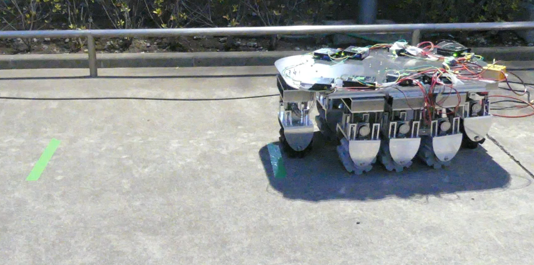
\includegraphics[width=0.8\textwidth]{zikkenn_image2.png}
  \vspace{2mm}
  \caption{Driving experiment on concrete}
  \label{zikkenn_image1_2}
\end{figure}

\begin{figure}[H]
  \centering
  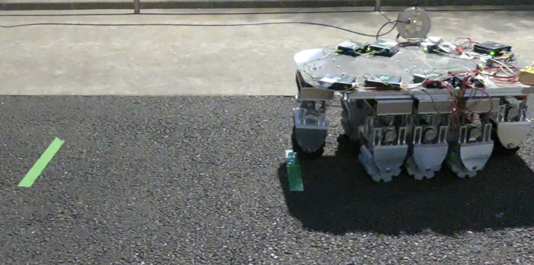
\includegraphics[width=0.8\textwidth]{zikkenn_image3.png}
  \vspace{2mm}
  \caption{Driving experiment on asphalt}
  \label{zikkenn_image1_3}
\end{figure}

\subsection{理論値の算出}
走行スピードはモータの性能とプログラムに依存する為, モータの性能から出される理論値との比較を行う. なお本機体は8輪でありモータにかかる負荷は均一ではない為, 今回の実験には機体重量によるモータへの負荷は考慮せず, また風などの外力も考慮しないものとする.

理論値は以下の式より算出する.

\begin{figure}[H]
  
\includegraphics[width=0.9\textwidth]{rironnti.png}
\end{figure}


\subsection{実験結果}

上記の実験より得られたデータを表 \ref{friction}に示す.
\vspace{-2mm}

\begin{table}[h]
    \centering
    \caption{Driving experiment}
    \scalebox{1.5}{
    \begin{tabular}{ccc}
    environment           & distance traveled      \\ \hline
    theoretical value     & 26.53 [mm/s]            \\
    iron plate            & 24.39 [mm/s]            \\
    concrete              & 25.64 [mm/s]            \\
    asphalt               & 26.32 [mm/s]
    \end{tabular}
    }
    \label{friction}
  \end{table}
    
実験の結果, 理論値にかなり近い走行性能を出せることが分かった.
これにより, 変形機構を搭載した事による平地での走行性能への影響はないと考えられる.

また, データより摩擦係数の高い環境ほど走行効率が高いことも示されている.


\newpage

\section{段差踏破実験}

車輪数の多い機体には段差踏破時のタイムロスが考えられる.
そのため, 踏破可能な高さの検証と, 高さの変化による走行時間の変化の検証を行うことで段差踏破性能の評価を行う.

\subsection{直進時の段差踏破実験}
直進時は, 進行方向に対して段差がある場合に車輪数による走行への影響を最も受ける可能性がある.
よって全ての車輪が段差を踏破するまでに生じるロスの検証を行う.

実験風景を図\ref{zikkenn_image2_1}, \ref{zikkenn_image2_2}に示す.

\begin{figure}[H]
  \centering
  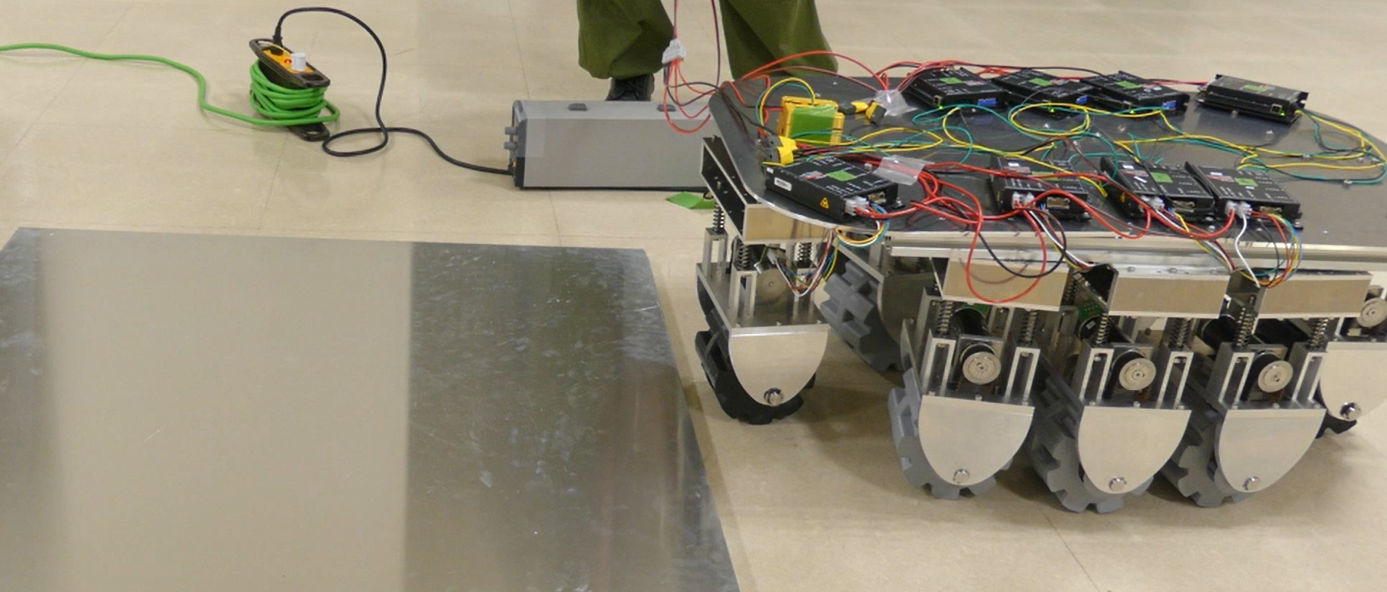
\includegraphics[width=0.8\textwidth]{zikkenn_image4.png}
  \vspace{2mm}
  \caption{Step-climbing experiment with straight motion1}
  \label{zikkenn_image2_1}
\end{figure}

\begin{figure}[H]
  \centering
  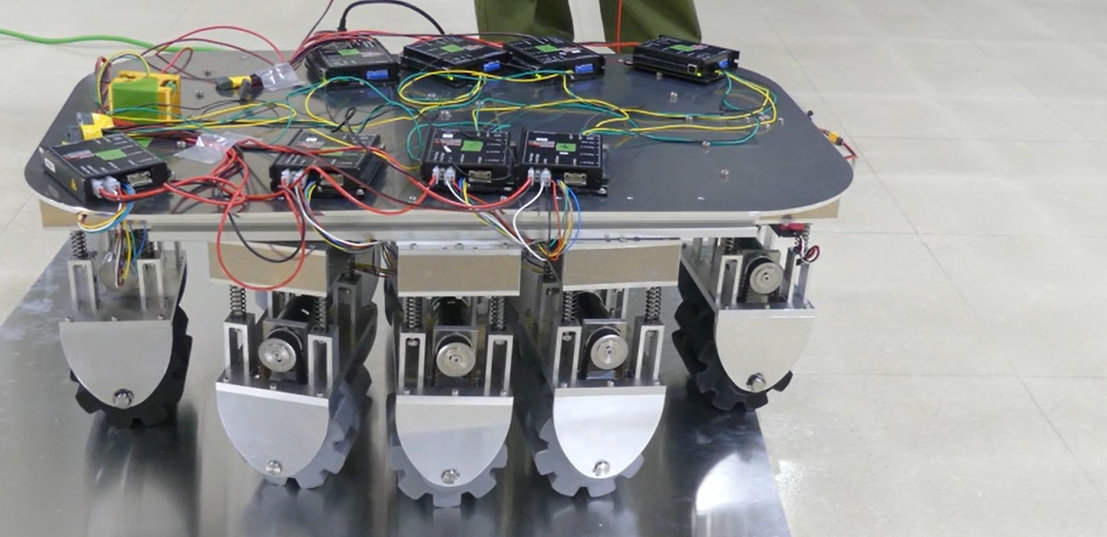
\includegraphics[width=0.8\textwidth]{zikkenn_image5.png}
  \vspace{2mm}
  \caption{Step-climbing experiment with straight motion2}
  \label{zikkenn_image2_2}
\end{figure}


\newpage
\subsection{旋回時の段差踏破実験}
旋回時の段差踏破は先行機体であるクローラ型移動ロボットでは不可能である.

本機体の有用性を証明するため, 機体の両側面に障害物を配置して踏破可能であるかの実験を行う.
また, 直進時と同様に車輪数による走行への影響の検証も行う.

実験風景を図\ref{zikkenn_image3_1}, \ref{zikkenn_image3_2}に示す.

\begin{figure}[H]
  \begin{minipage}{0.45\hsize}
    \centering
    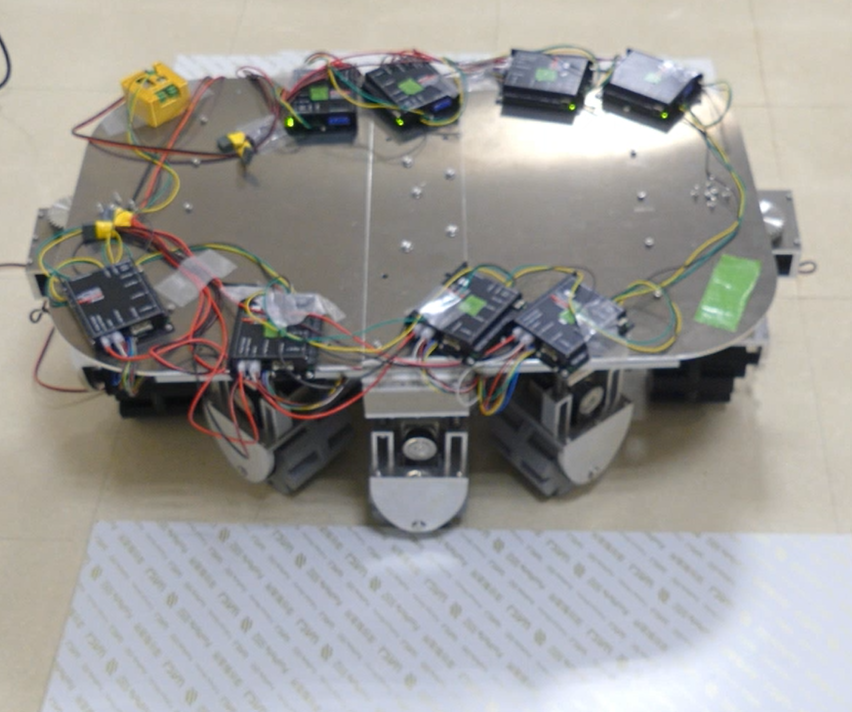
\includegraphics[height=60mm]{zikkenn_image6.png}
    \caption{Step-crossing experiment using turning motion1}
    \label{zikkenn_image3_1}
  \end{minipage}
  \begin{minipage}{0.5\hsize}
    \centering
    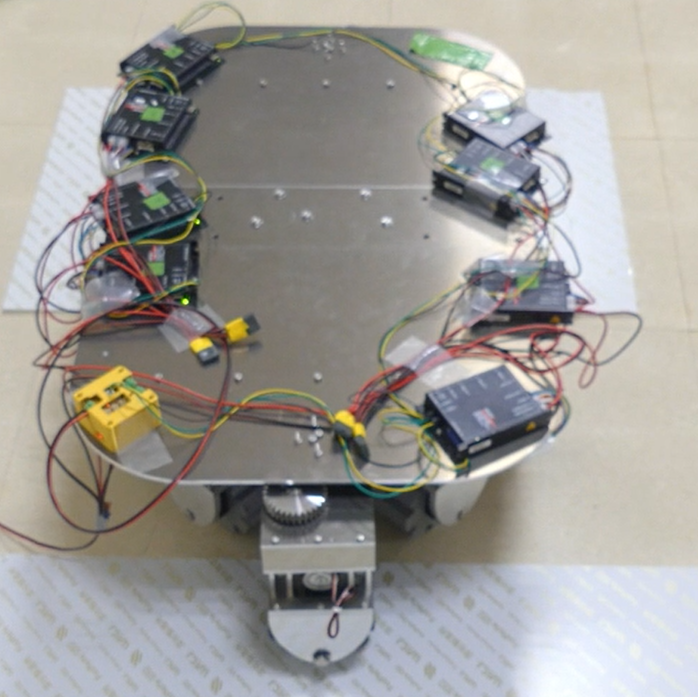
\includegraphics[height=60mm]{zikkenn_image7.png}
    \caption{Step-crossing experiment using turning motion2}
    \label{zikkenn_image3_2}
  \end{minipage}
\end{figure}


\subsection{実験結果}
上記の実験より得られたデータを表 \ref{friction2}に示す.
\vspace{-2mm}

\begin{table}[h]
    \centering
    \caption{Step-crossing experiment}
    \scalebox{1.5}{
    \begin{tabular}{ccc}
    step height    & crossing time     & turning time  \\ \hline
    0 [mm]          & 32 [s]       & 26 [s]          \\
    6 [mm]          & 32 [s]       & 24 [s]          \\
    12 [mm]         & 33 [s]       & 28 [s]          \\
    18 [mm]         & 32 [s]       & 27 [s]          \\
    24 [mm]         & 34 [s]       & 29 [s]
    \end{tabular}
    }
    \label{friction2}
\end{table}

実験の結果, 本機体では直進時の段差踏破は可能であり, またクローラ型移動ロボットでは踏破不可能な機体両側面の段差も問題なく踏破可能であった.

また実験データより, 直進時と旋回時どちらも段差の高さによる走行スピードへの影響はほとんど無かった.
これは, サスペンション機構を搭載し上下方向に自由度を持たせることで, タイムロスを抑える事ができたと考えられる.









%第3章
\newpage
\part{結論}

\section{まとめ}
本研究では泥濘地でのスタックを防止するため, 各車輪の方向を進行方向にそろえる機構をもつ8輪運搬ロボットの提案と製作を行った.
また現場ヤードを想定した検証を行った.
    
検証の結果, 平地走行や段差踏破では十分な性能を持つことが検証できた.
よって本機体の有用性を証明する事ができたと言える.


\section{今後の展望}
今後は以下に示した土地盤で含水率を変えつつ走行実験を行い, 泥濘地において車輪を使用した機体の有用性の評価と, 方向可変な車輪のスタック防止に対する有用性の評価を行う必要がある.

\begin{itemize}
  \item 礫
  \item 砂
  \item シルト
  \item 粘土
\end{itemize}

\section{発展的な展望}
本機体の車輪形状は, 想定される様々な環境に合う設計にしているが, あくまでも創造しうる範囲での設計である.

本研究で現場ヤードでの走行性能を示す事はできたが, 今回の車輪形状が最適である証明はできていない.最適な形状を証明するには, いくつかの形状を製作し比較実験を行う必要がある.
また, 今回泥濘地での走行実験は行えていない為, 泥濘地において最適な車輪形状の検討も必要である.

さらに泥濘地での実験結果しだいでは, 車輪を使用した機体の1番の難点である, 接地面積の少なさを改善する必要が出てくる可能性もある.
よって, 接地面積増加を目標とした新機構の考案も視野に入れて今後の研究を進める必要がある.







%参考文献
\newpage
\begin{thebibliography}{99}
\addcontentsline{toc}{section}{参考文献}

\setlength{\itemsep}{-2pt} 
\bibitem{ref1} IH塗膜除去工法研究会: IH塗膜除去工法の概要, 
\url{http://ih-tmk.com} (2026.1.27参照).
\bibitem{ref2} 綱川大悟, 米田完, 中原智法: 壁面走行ロボットの開発, 日本機械学会ロボメカ講演会論文集 (2021), 
\url{https://www.jstage.jst.go.jp/article/jsmermd/2021/0/2021_2P1-A12/_article/-char/ja/} (2026.1.27参照).

\end{thebibliography}

%謝辞
%謝辞
\lhead {}   %:天左側ヘッダの定義
\newpage
\rhead {謝辞}   %:天右側ヘッダの定義
\section* {謝辞}
\addcontentsline {toc} {section} {謝辞}
\vspace {5mm}

本研究を進めるにあたりご指導くださいました米田完教授に謹んで感謝の意を表します. 先生の多くのご助言があったからこそ, ここまで研究を進めることができました. 


共同研究先であるオリエンタル白石株式会社の松村様, 倉知様, 進藤様, 岩崎様にも大変お世話になりました.
また倉知様には特別講義として地盤講習会を開いてくださった事, 心より感謝申し上げます。

株式会社ミスミ様には私の拙い図面や加工指示に基づき, 多くの部品を製作していただきました. 感謝申し上げます. 


また, 米田研究室の皆様にも日ごろから実験や製作の手伝いをして頂きました. また, 助言もいただきました. 心より感謝します.


最後に, 大学に進む機会を与えてくださり, あらゆる面で支えてくださった両親にこの場を借りて感謝申し上げます.
\pagenumbering{alph}
\clearpage

\setcounter{page}{1}
\pagenumbering{alph}

%\includepdf[pages={-},nup=1x2]{pdf/A_body_plan.pdf}

%\includepdf[pages={-}]{pdf/F_test_of_const.pdf}

%\includepdf[pages={-}]{pdf/G_NSC0058_SPEC.pdf}
%\includepdf[pages={-}]{pdf/H_NSC0075_SPEC.pdf}

\end{document}